\documentclass[11pt]{article}
\usepackage{mathtools}
\usepackage{amssymb}
\usepackage{amsthm}
\usepackage{polski}
\usepackage[utf8]{inputenc}
\usepackage{geometry}
\usepackage{mnsymbol}
\usepackage{graphicx}
\usepackage{textgreek}
\usepackage{float}
\usepackage{caption}
\author{Łukasz Jezapkowicz}
\title{Tranzystor unipolarny}
\date{10.05.2019}
\begin{document}
\newgeometry{tmargin=2cm,bmargin=2cm,lmargin=2cm,rmargin=2cm}
\maketitle
\tableofcontents \newpage
\section{Wyznaczenie wartości napięcia progowego $U_T$ tranzystora unipolarnego}
\subsection{Cel ćwiczenia}
Celem ćwiczenia było zapoznanie się z prostym obwodem elektrycznym zawierającym tranzystor unipolarny oraz wyznaczenie wartości napięcia progowego $U_T$ tranzystora
unipolarnego typu NMOS.
\subsection{Przebieg ćwiczenia}
Na pulpicie symulacyjnym zbudowałem obwód elektryczny widoczny na \textbf{Rys. 1}. Przedstawiony poniżej układ zawiera źródło napięcia $V_{DD}=12V$, rezystor $R_1 = 1k\Omega$ oraz tranzystor unipolarny $IRF540$ typu NMOS. Do układu podłączyłem również oscyloskop dzięki, któremu zbadam zależności napięcia sterującego $U_{GS}$ i napięcia $U_{DS}$ na drenie tranzystora. Na bramkę tranzystora podałem sygnał liniowo narastający o niskiej częstotliwości - sygnał trójkątny o parametrach : częstotliwości równej $10Hz$, wypełnienia równego $50\%$ oraz amplitudy $12V$.
\begin{figure}[H]
\centering
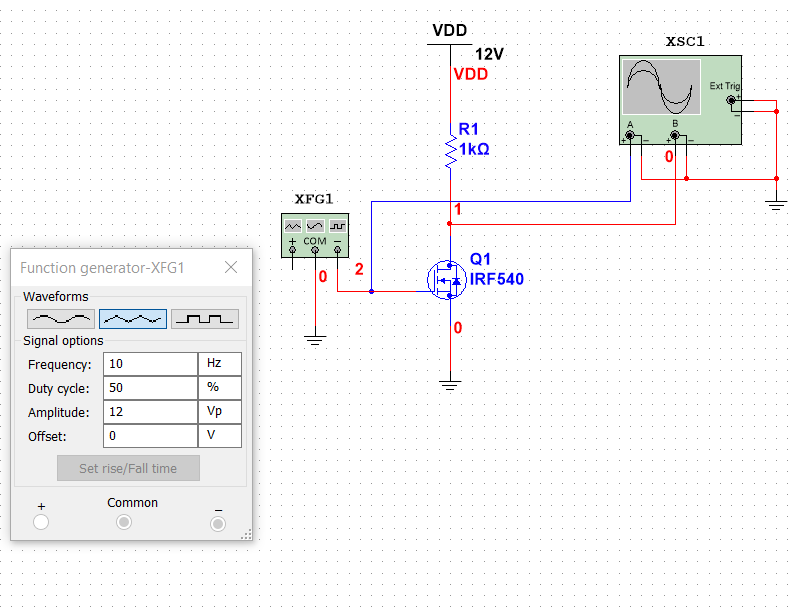
\includegraphics[width=10cm]{a37}
\caption*{\textbf{Rys. 1}: Schemat obwodu elektrycznego z tranzystorem typu NMOS z podłączonym oscyloskopem oraz liniowo narastającym sygnałem trójkątnym. }
\end{figure}
\noindent Przy użyciu ekranu oscyloskopu oraz analizy Transient odczytałem punkt przecięcia przebiegu wejściowego narastającego liniowo i przebiegu wyjściowego z drenu tranzystora. Odczytany punkt to nasze poszukiwane napięcie progowe $U_T$. Ekran oscyloskopu oraz wyniki analizy Transient widać odpowiednio na \textbf{Rys. 2} oraz \textbf{Rys. 3}. Przy użyciu analizy Transient odczytałem wartość $U_T = 3.5544 V $.
\begin{figure}[H]
\centering
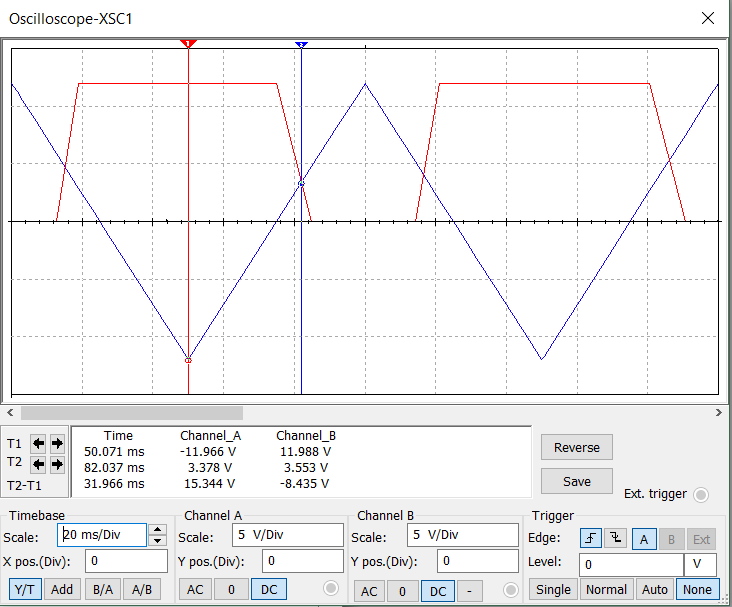
\includegraphics[width=10cm]{a38}
\caption*{\textbf{Rys. 2}: Ekran oscyloskopu dla obwodu elektrycznego widocznego na Rys. 1. Wskaźnik numer 2 wyznacza napięcie progowe $U_T$ tranzystora. }
\end{figure}
\begin{figure}[H]
\centering
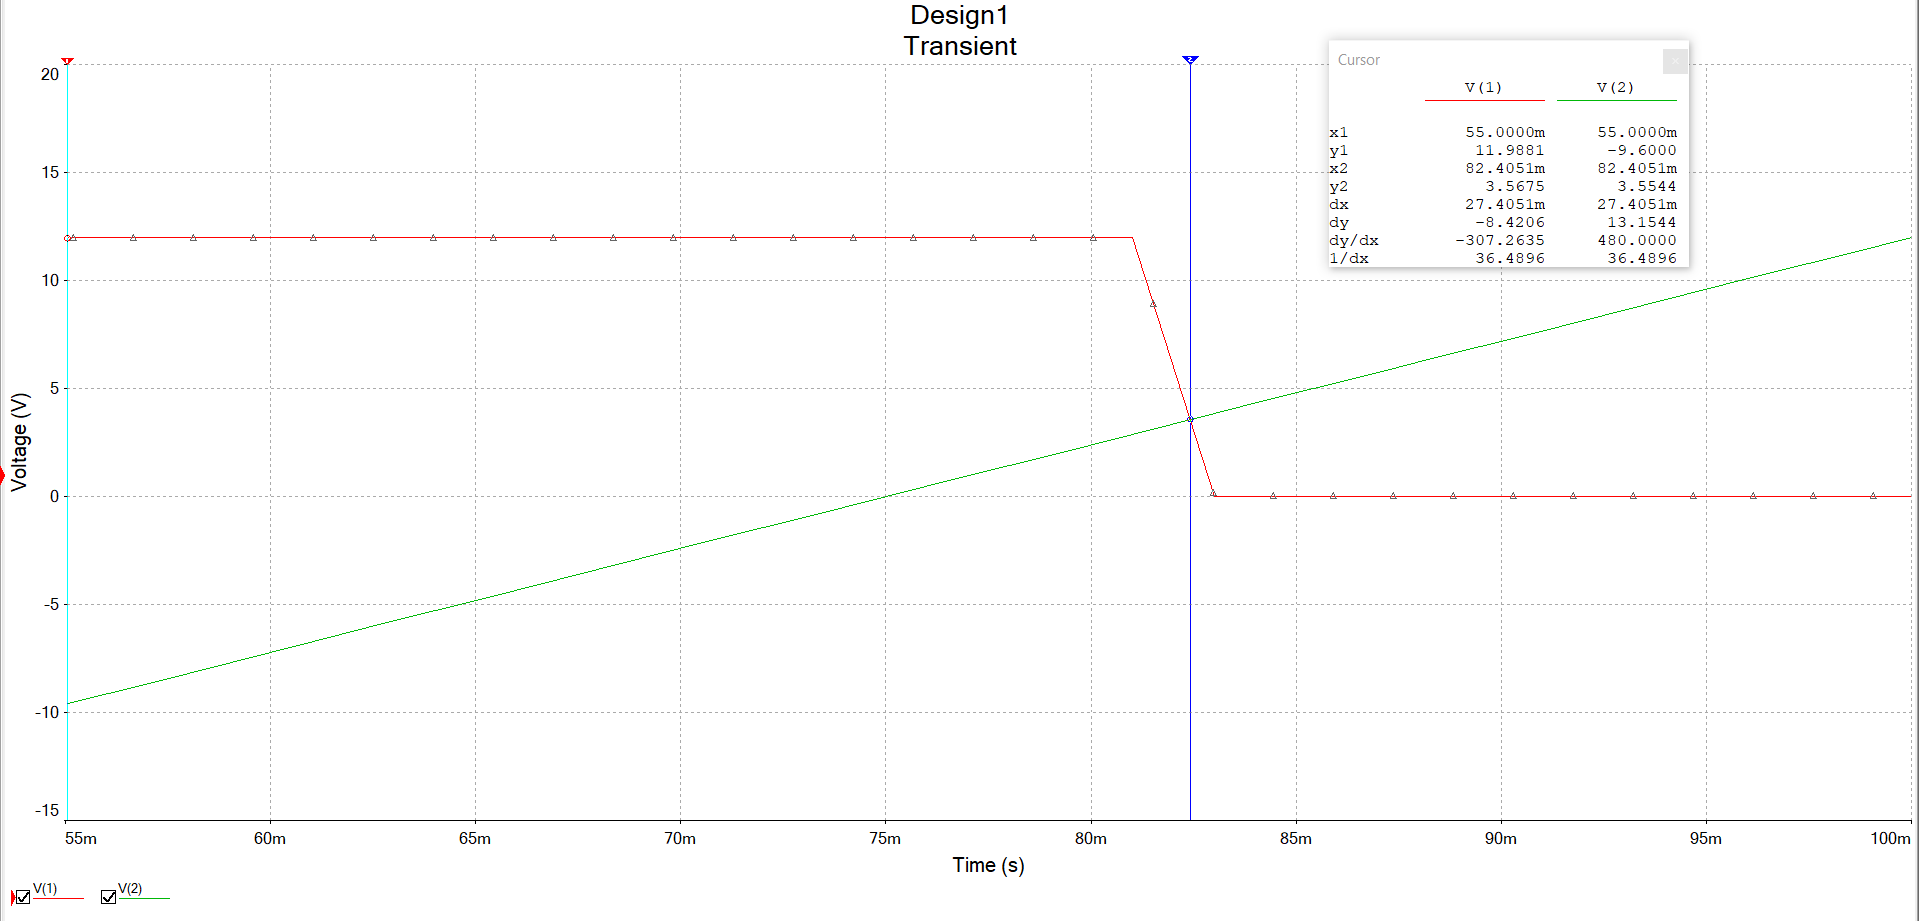
\includegraphics[width=10cm]{a39}
\caption*{\textbf{Rys. 3}: Wyniki analizy Transient dla obwodu elektrycznego widocznego na Rys. 2. Wskaźnik numer 2 wyznacza napięcie progowe $U_T$ tranzystora. }
\end{figure}
\subsection{Wnioski}
Po przekroczeniu wartości napięcia progowego $U_T$ w tranzystorze zaczyna płynąć coraz większy prąd $I_D$ a więc napięcie wyjściowe $U_{WY}$ zgodnie z wzorem $U_{WY} = U_{DD} - I_D*R_D$ maleje. Analiza przebiegu napięcia wejściowego
i wyjściowego pozwala na dokładne wyznaczenie wartości napięcia progowego.
\section{Tranzystor unipolarny w układzie wzmacniacza sygnałów zmiennych}
\subsection{Cel ćwiczenia}
Celem ćwiczenia było zapoznanie się z prostym obwodem elektrycznym zawierającym tranzystor w układzie wzmacniacza sygnałów zmiennych i wyznaczenie punktu pracy $Q(U_{DS},I_D)$ oraz wartości transkonduktancji $g_m$ i wzmocnienia
napięciowego $k_u$.
\subsection{Przebieg ćwiczenia}
Na \textbf{Rys.4} zamieściłem bazowy układ wzmacniacza sygnałów zmiennych z tranzystorem unipolarnym NMOS $IRF540$.
\begin{figure}[H]
\centering
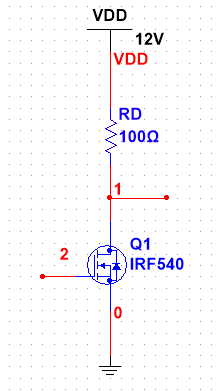
\includegraphics[width=4cm]{a40}
\caption*{\textbf{Rys. 4}: Bazowy układ wzmacniacza sygnałów zmiennych z tranzystorem unipolarnym NMOS $IRF540$.}
\end{figure}
\noindent Używając prawa Ohma i praw Kirchhoffa można obliczyć punkt pracy $Q(U_{DS},I_D)$. Do obliczenia punktu pracy użyłem następujących podstawowych zależności dotyczących działania tranzystora w obwodzie:
$U_{Wy} = \frac{U_{DD}}{2} = U_{DS}$ oraz $I_D = \frac{U_{DD}-U_{Wy}}{R_D}$. Po podstawieniu wartości z obwodu na \textbf{Rys. 4}: $U_{Wy} = \frac{12V}{2} = 6V$, $I_D = \frac{12V-6V}{100\Omega} = 60mA$. \newline
Następnie na pulpicie symulacyjnym zbudowałem układ widoczny na \textbf{Rys. 5} zawierający źródło napięcia o wartości $12V$, dwa rezystory $R_D = 100\Omega$ oraz $R_1 = 8.5k\Omega$, 3 potencjonometry $R_2 = 3k\Omega$,
$R_3 = 1k\Omega$ oraz $R_4 = 100\Omega$, tranzystor unipolarny typu NMOS oraz 3 podłączone multimetry, dzięki którym mogłem zmierzyć $U_{Wy}$, $I_D$ oraz opór zastępczy trzech potencjometrów. Potencjometry ustawiłem empirycznie 
w taki sposób by wyniki pomiarów zgadzały się z wyliczonym wcześniej punktem pracy $Q(6V,60mA)$.
\begin{figure}[H]
\centering
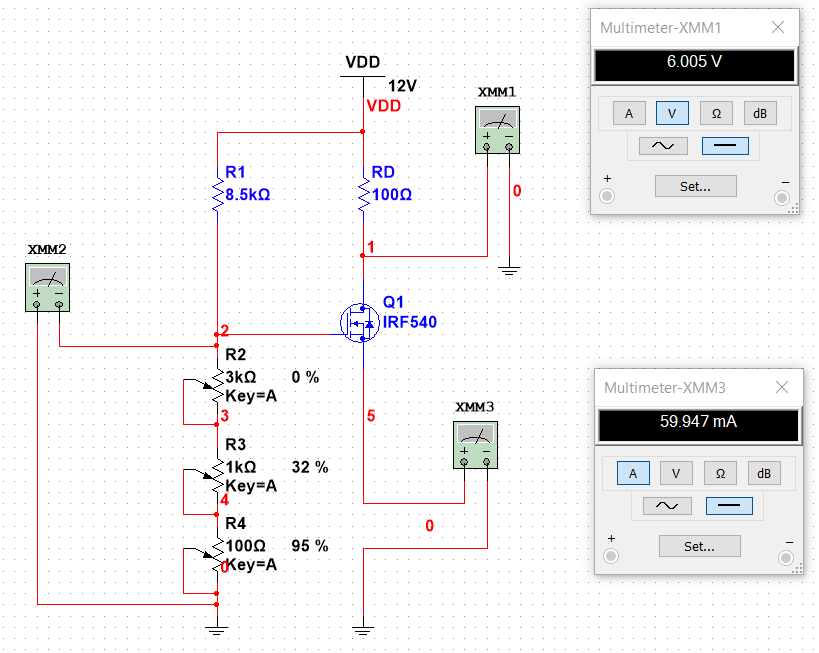
\includegraphics[width=10cm]{a41}
\caption*{\textbf{Rys. 5}: Schemat obwodu elektrycznego z tranzystorem NMOS, źródłem napięcia $V_{DD}$, dwoma rezystorami $R_D$,$R_1$ oraz 3 potencjonometrami $R_2$,$R_3$ oraz $R_4$ tworzącymi potencjometryczny układ polaryzacji.}
\end{figure}
\noindent Następnie obliczyłem obwód zastępczy trzech potencjometrów przy pomocy multimetru $XMM2$ co widać na \textbf{Rys. 6}. Obliczony opór zastępczy zastąpiłem jednym rezystorem $R_2$ o wartości rezystancji $3.685k\Omega$. Zmiana ta niemal nie zmieniła wartości $U_{Wy}$ oraz $I_D$ w obwodzie więc nie zmieniałem wartości oporu wskazanego przez multimetr $XMM2$. Obwód z rezystorem $R_2$ widać na \textbf{Rys. 7}.
\begin{figure}[H]
\centering
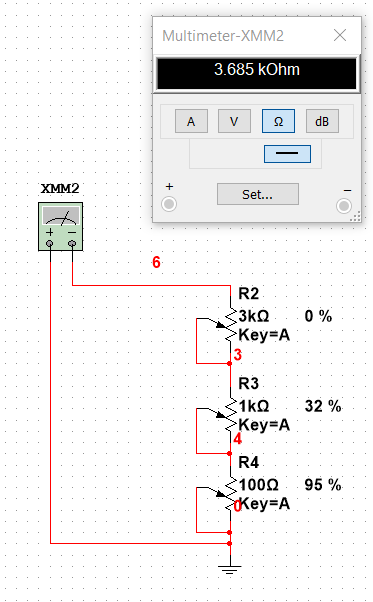
\includegraphics[width=5cm]{a42}
\caption*{\textbf{Rys. 6}: Układ trzech potencjometrów $R_2$, $R_3$, $R_4$ z obliczonym oporem zastępczym.}
\end{figure}
\begin{figure}[H]
\centering
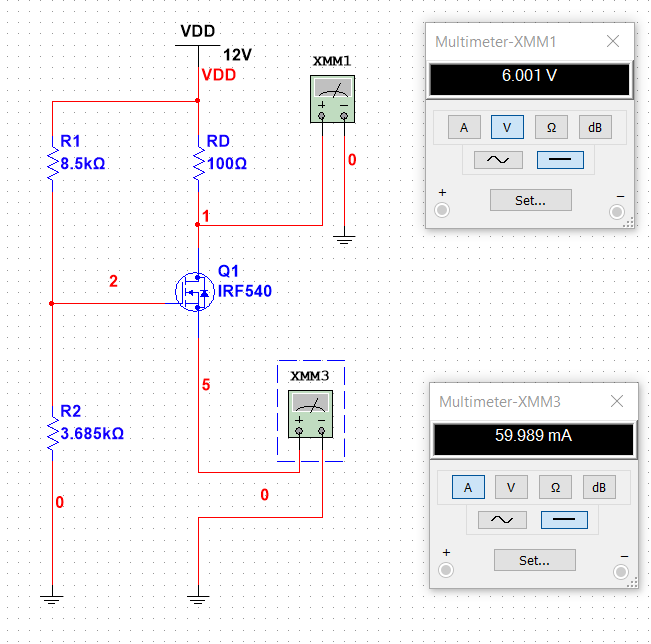
\includegraphics[width=10cm]{a43}
\caption*{\textbf{Rys. 7}: Schemat obwodu elektrycznego z tranzystorem NMOS, źródłem napięcia $V_{DD}$ i trzema rezystorami $R_D$,$R_1$ oraz $R_2$, który zastąpił wcześniejsze potencjometry. }
\end{figure}
\noindent Następnie do obwodu z \textbf{Rys. 7} podłączyłem multimetr $XMM2$ pozwalający zmierzyć $U_{GS}$, którego zmierzoną wartość $3.629V$ użyłem do obliczenia transkonduktancji używając wzoru: $g_m = \frac{I_D}{U_{GS}}=
\frac{59.974mA}{3.629V} = 0.0165S$.
\begin{figure}[H]
\centering
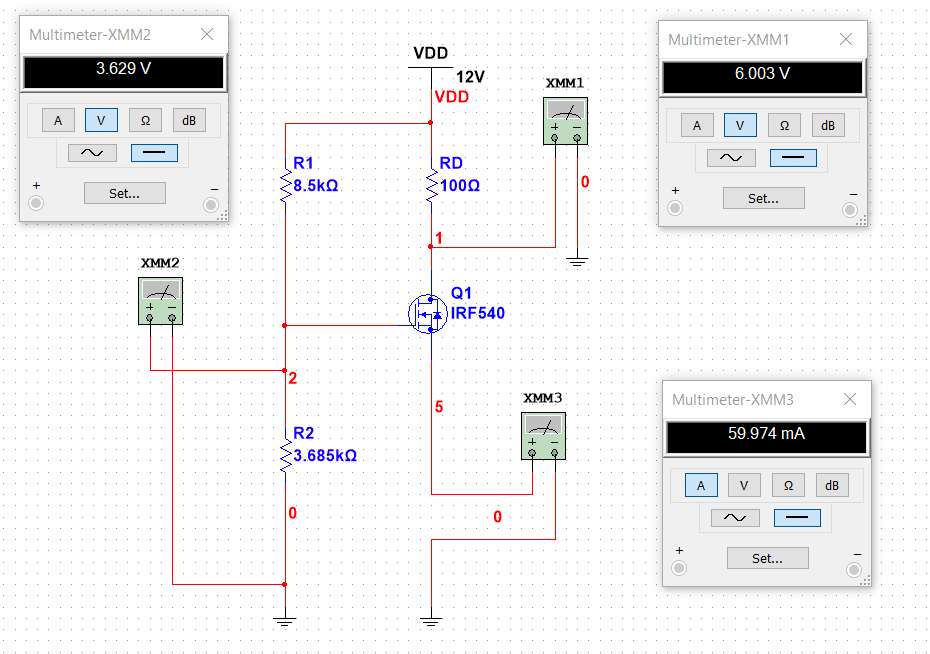
\includegraphics[width=10cm]{a44}
\caption*{\textbf{Rys. 8}: Schemat obwodu elektrycznego z Rys. 7 z podłączonym multimetrem mierzącym $U_{GS}$. }
\end{figure}
\noindent Na koniec w celu obliczenia wzmocnienia napięciowego $k_u$ dołączyłem do obwodu generator - źródło sygnału zmiennego $XFG1$ o parametrach: częstotliwośc $1kHz$, amplituda $100mV$, składowa stała $0V$. Do obwodu dołączyłem również kondensator $C_1 = 100nF$ oraz oscyloskop $XSC1$, do którego podłączyłem sygnał z generatora oraz z drenu tranzystora.
\begin{figure}[H]
\centering
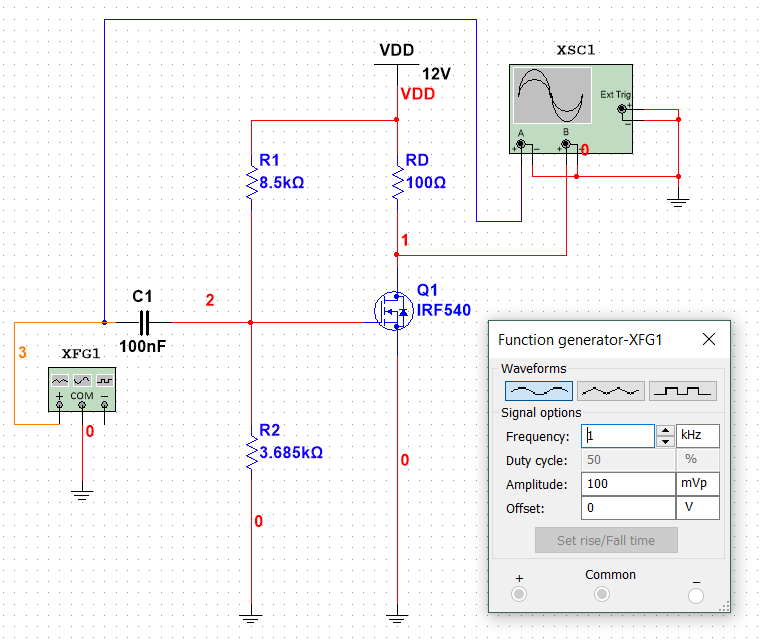
\includegraphics[width=10cm]{a45}
\caption*{\textbf{Rys. 9}: Schemat obwodu elektrycznego z źródłem sygnału zmiennego $XFG1$ oraz dołączonym oscyloskopem $XSC1$. }
\end{figure}
\noindent Do obliczenia wzmocnienia napięciowego $k_u$ posłużyłem się wzorem $k_u = \frac{{\Delta}u_{wy}}{{\Delta}u_{we}}$. W tym celu obliczyłem podwojoną amplitudę sygnału wyjściowego równą $-10.57V$ oraz podwojoną amplitudę sygnału wejściowego równą $199.972mV$. Wyniki takie otrzymałem dzięki pomiarom z analizy Transient widocznym na \textbf{Rys. 10} oraz \textbf{Rys. 11}. Ponieważ sygnał wejściowy i wyjściowy są względem siebie obrócone to do zmiany sygnału wyjściowego dołączyłem znak minus. Obliczona wartość wzmocnienia napięciowego: $k_u = \frac{-10.57V}{199.972mV} = -52.8614$.
\begin{figure}[H]
\centering
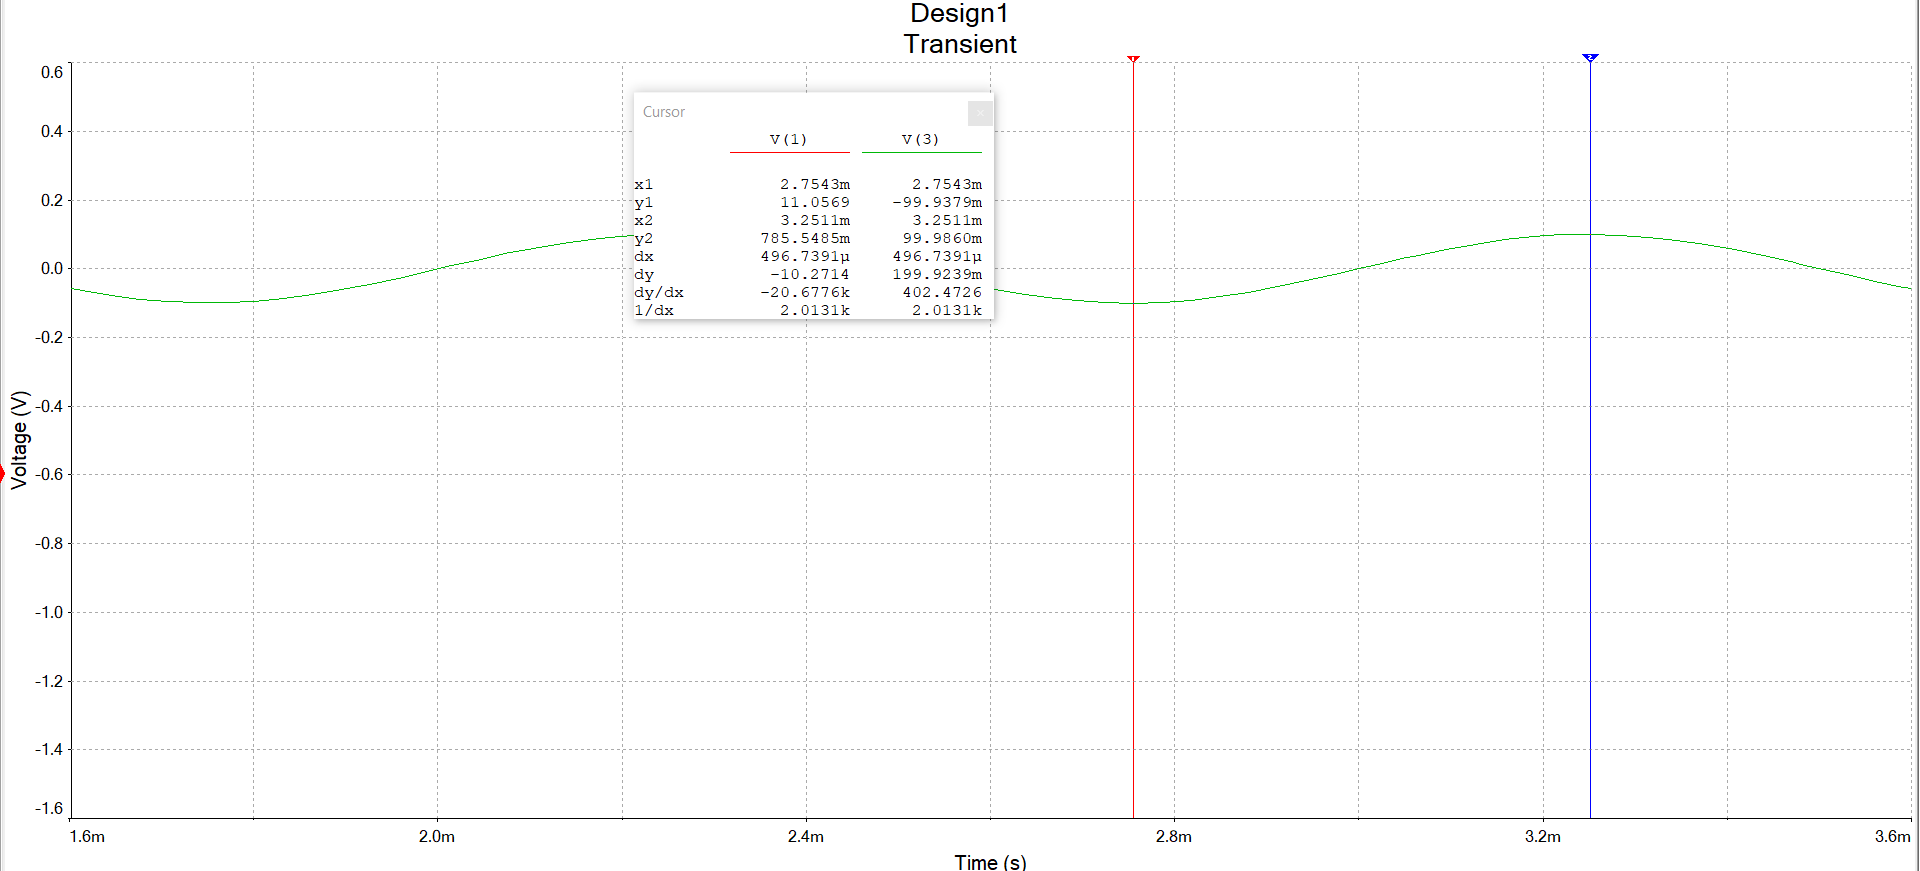
\includegraphics[width=10cm]{a48}
\caption*{\textbf{Rys. 10}: Pomiary analizy Transient z zaznaczonymi punktami napięcia wejściowego pozwalającymi obliczyć podwojoną amplitude sygnału wejściowego. }
\end{figure}
\begin{figure}[H]
\centering
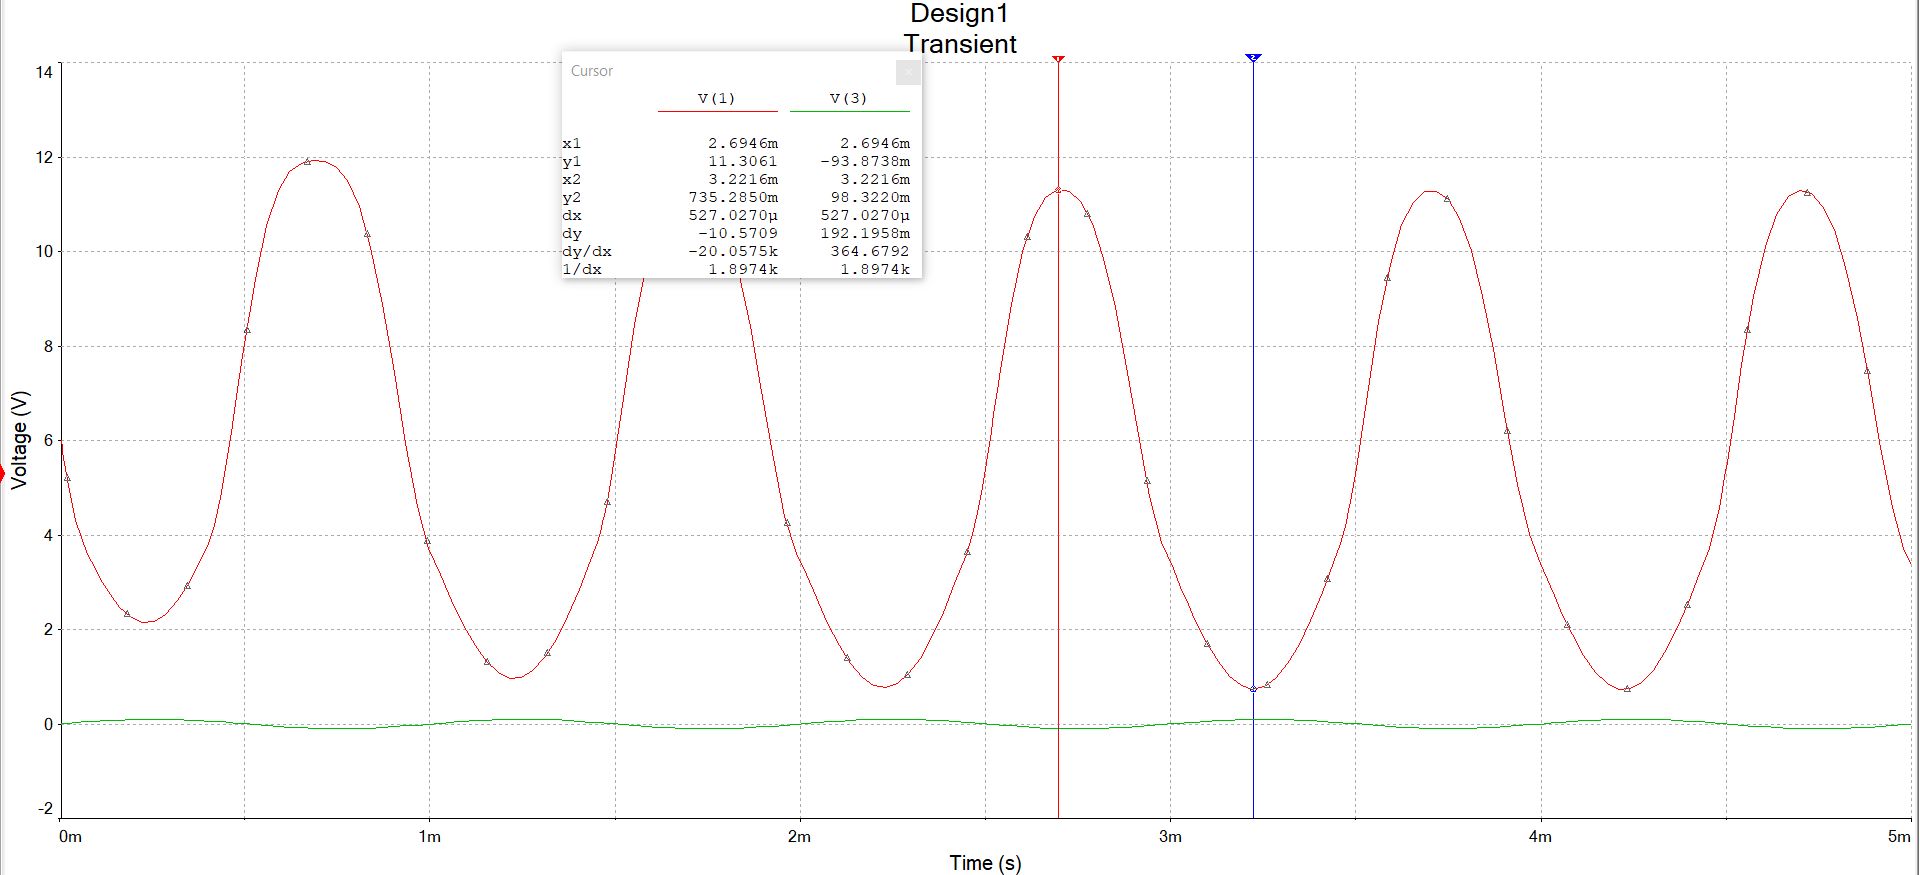
\includegraphics[width=10cm]{a47}
\caption*{\textbf{Rys. 11}: Pomiary analizy Transient z zaznaczonymi punktami napięcia wyjściowego pozwalającymi obliczyć podwojoną amplitude sygnału wyjściowego.  }
\end{figure}
\noindent Wszelkie obliczenia zawarte w tym ćwiczeniu umieściłem w tabeli widocznej na \textbf{Rys.12}.
\begin{figure}[H]
\centering
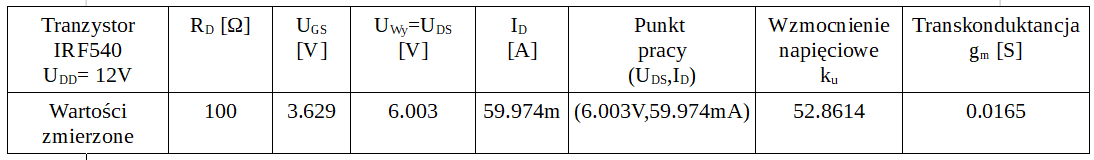
\includegraphics[width=10cm]{a49}
\caption*{\textbf{Rys. 12}: Tabela zawierająca wszystkie obliczone wartości w układzie w ćwiczeniu. }
\end{figure}
\subsection{Wnioski}
Do sterowania składową stałą sygnału można skutecznie użyć dzielnika napięcia. Użyte w ćwiczeniu potencjometry pozwoliły skutecznie obliczyć opór zastępczy, który pozwolił osiągnąć szukany punkt pracy $Q$. W ćwiczeniu zaobserowaliśmy również 
odwrócenie sygnału wejściowego oraz jego wzmocnienie, policzyliśmy również charakterystyczne parametry obwodu: wzmocnienie napięciowe oraz transkonduktancję.
\section{Tranzystor unipolarny jako klucz przełączający}
\subsection{Cel ćwiczenia}
Celem ćwiczenia była obserwacja działania tranzystora unipolarnego jako klucza przełączającego przy pomocy prostego obwodu eletrycznego i zmierzenie czasów włączania i wyłączania tranzystora.
\subsection{Przebieg ćwiczenia}
Na pulpicie symulacyjnym zbudowałem obwód elektryczny tranzystora unipolarnego pracującego jako klucz przełączający zawierający tranzystor unipolarny NMOS, dwa rezystory $R_1=10\Omega$ oraz $R_2=100\Omega$ oraz źródło napięcia stałego
o wartości $V_1=12V$. Do układu podłączyłem również generator $XFG1$ z sygnałem prostokątnym o częstotliwości $50kHz$ i współczynniku zapełnienia $50\%$ oraz oscyloskop $XSC1$. Układ widoczny jest na \textbf{Rys.13}.
\begin{figure}[H]
\centering
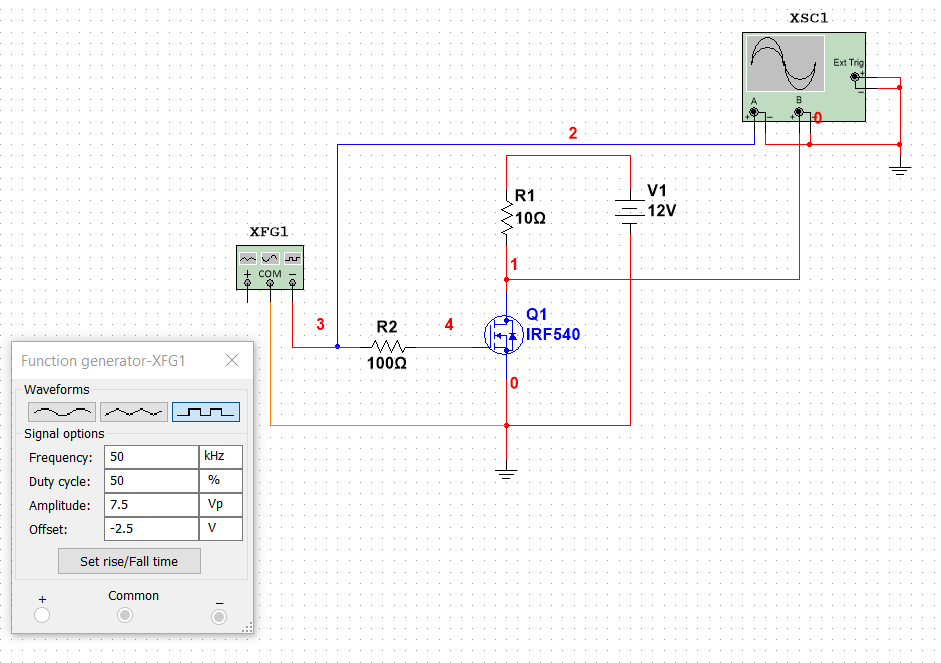
\includegraphics[width=10cm]{a50}
\caption*{\textbf{Rys. 13}: Schemat obwodu elektrycznego z tranzystorem unipolarnym pracującym jako klucz przełączający. }
\end{figure}
\noindent Wartości amplitudy i offset'u generatora należało wybrać w taki sposób by górny poziom napięcia wejściowego $E_F$ oraz dolny poziom napięcia wejściowego $E_R$ były zgodne z wartościami widocznymi w tabeli na \textbf{Rys. 16}. Do wyznaczenia
odpowiednich wartości użyłem ekranu oscyloskopu, na którym w łatwy sposób mogłem obserwować wartości górnego i dolnego poziomu napięcia. \newline
Następnie zmierzyłem czasy włączenia i wyłączenia tranzystora dla każdej kombinacji parametrów z tabeli. Do obliczenia ich użyłem analizy Transient. Czas włączania $t_{ON} = t_{d(on)}+t_r$, gdzie $t_{d(on)}$ to czas opóźnienia włączenia tranzystora
(delay time) czyli czas pomiędzy początkiem impulsu wejściowego a chwilą gdy prąd drenu jest równy $10\%$ swojej wartości max (w tym przypadku oznacza to napięcie wyjściowe $10.8V$) zaś $t_r$ to czas narastania prądu drenu od $10\%$ do
 $90\%$ wartości max (oznacza to spadek napięcia wyjściowego z $10.8V$ do $1.2V$). Zadanie można więc uprościć mierząc czas od początku impulsu wejściowego do osiągnięcia wartości napięcia wyjściowego $1.2V$. Odpowiedni pomiar widać na
\textbf{Rys. 14}: $t_{ON} = 368.8178ns$. Czas wyłączania $t_{OFF} = t_{d(off)}+t_f$, gdzie $t_{d(off)}$ to czas opóźnienia wyłączenia tranzystora
(delay time) czyli czas pomiędzy końcem impulsu wejściowego a chwilą gdy prąd drenu jest równy $90\%$ swojej wartości max (w tym przypadku oznacza to napięcie wyjściowe $1.2V$) zaś $t_r$ to czas opadania prądu drenu od $90\%$ do $10\%$ wartości max (oznacza to wzrost napięcia wyjściowego z $1.2V$ do $10.8V$). Zadanie można więc uprościć mierząc czas od końca impulsu wejściowego do osiągnięcia wartości napięcia wyjściowego $10.8V$. Odpowiedni pomiar widać na
\textbf{Rys. 15}: $t_{OFF} = 403.7838ns$. 
\begin{figure}[H]
\centering
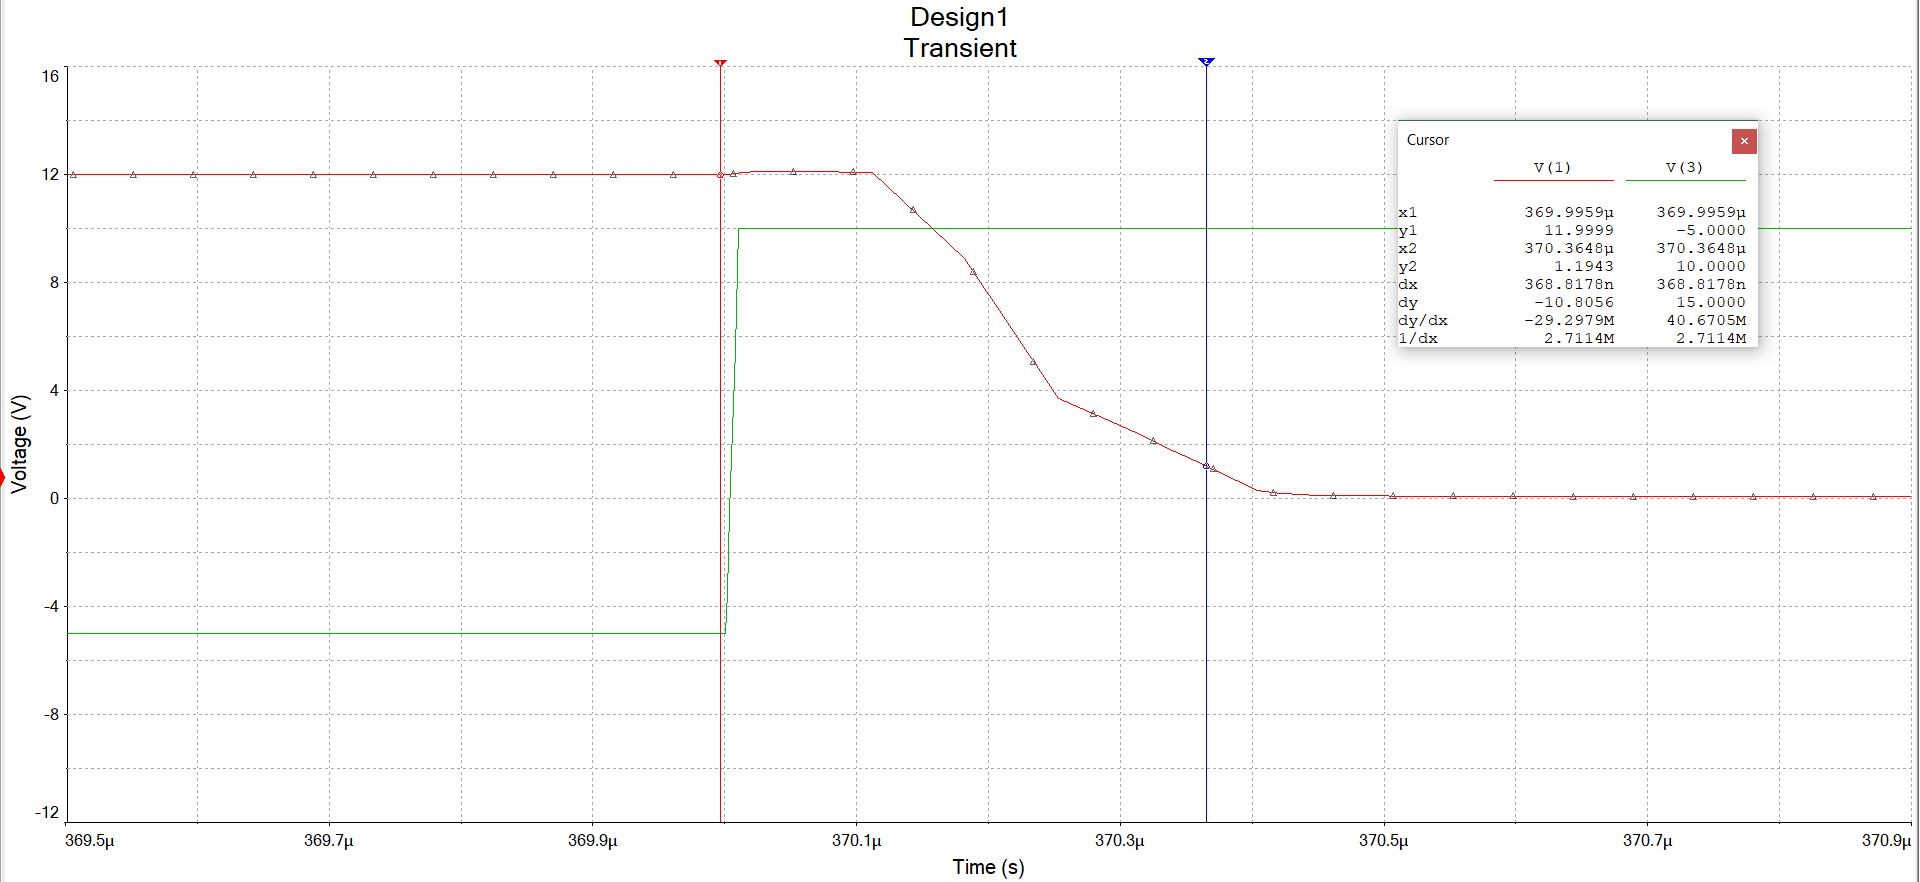
\includegraphics[width=10cm]{a51}
\caption*{\textbf{Rys. 14}: Analiza Transient pozwalająca znaleźć czas włączania tranzystora. Wynik należy odczytać z tabelki ze zmiennej dx. }
\end{figure}
\begin{figure}[H]
\centering
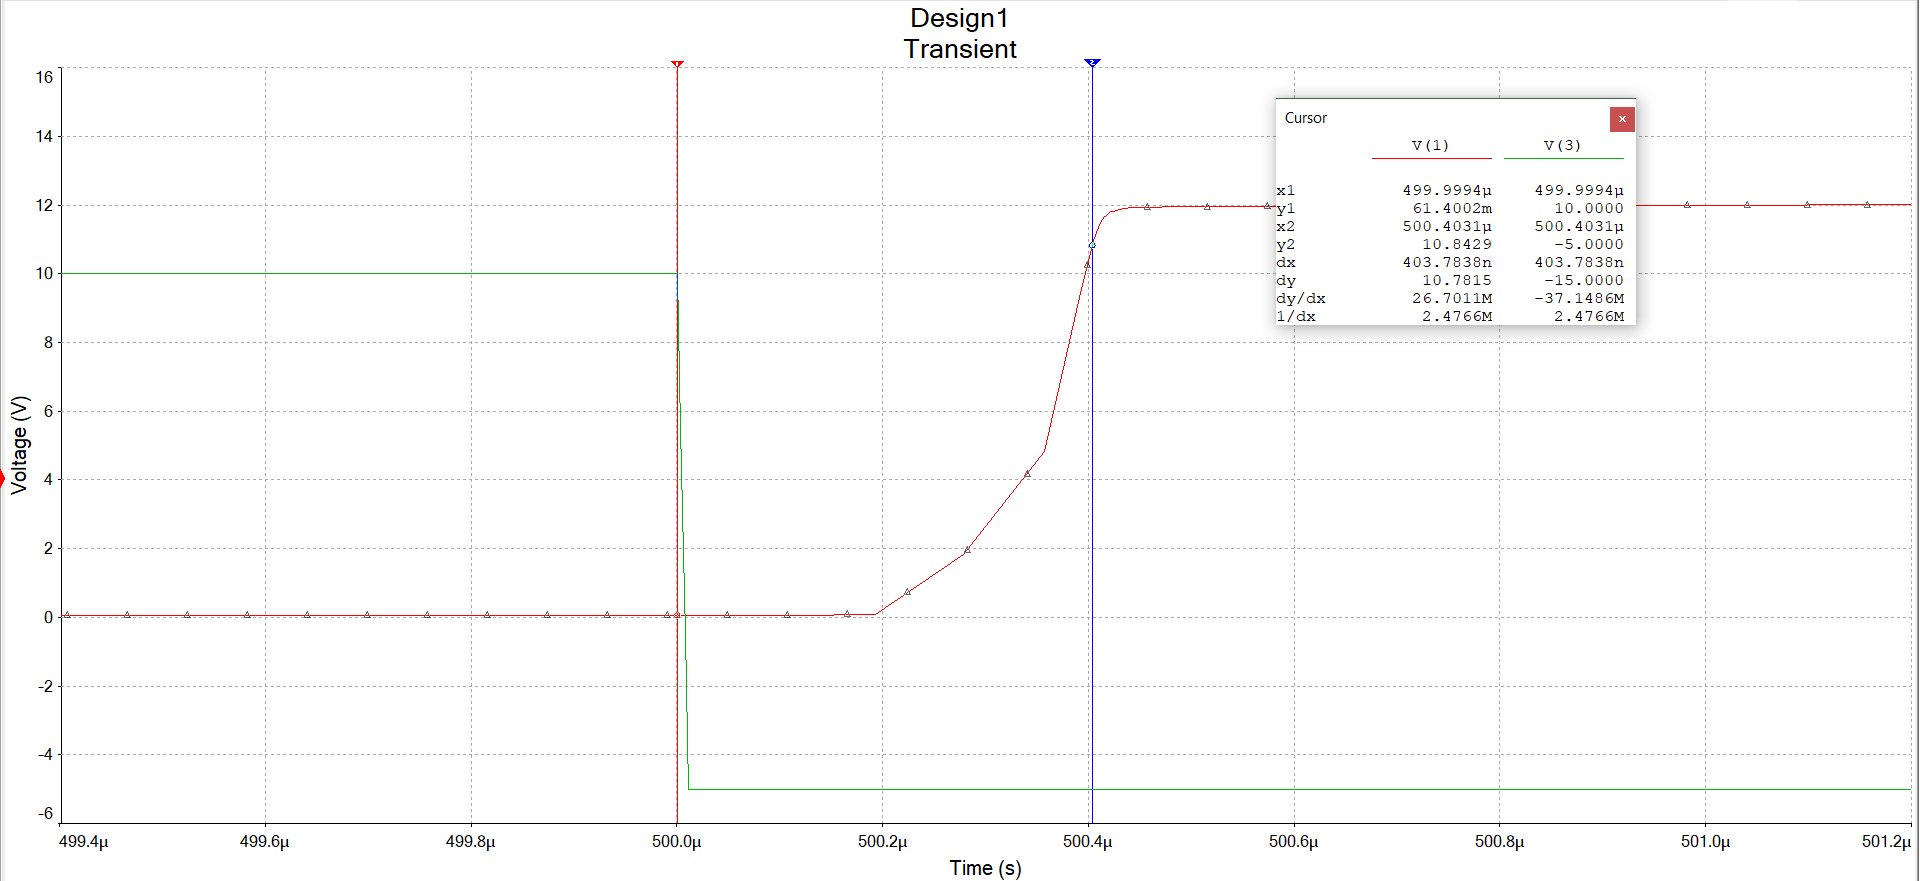
\includegraphics[width=10cm]{a52}
\caption*{\textbf{Rys. 15}: Analiza Transient pozwalająca znaleźć czas wyłączania tranzystora. Wynik należy odczytać z tabelki ze zmiennej dx. }
\end{figure}
\noindent Resztę przypadków zmierzyłem w ten sam sposób. Wszystkie zmierzone wartości widać w tabeli na \textbf{Rys. 16}.
\begin{figure}[H]
\centering
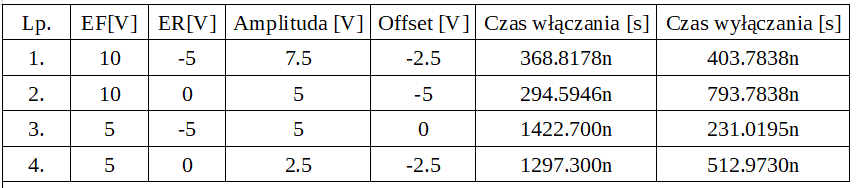
\includegraphics[width=10cm]{a53}
\caption*{\textbf{Rys. 16}: Tabela podsumowująca ćwiczenie z wszystkimi zmierzonymi wartościami czasów włączania i wyłączania. }
\end{figure}
\subsection{Wnioski}
Wykonane ćwiczenie pokazuje, że odpowiedni układ z tranzystorem można skutecznie stosować jako klucz przełączający. W ćwiczeniu obliczyliśmy również wartości czasu włączania i wyłączania tranzystora dla różnych górnych i dolnych poziomów napięcia wejściowego $E_R$ oraz $E_F$. Ćwiczenie pokazało, że dla różnych wartości obliczone czasy znacznie się różnią.
\section{Wstęp do układów logicznych}
\subsection{Cel ćwiczenia}
Celem ćwiczenia było zapoznanie się z prostym układem logicznym zbudowanym z tranzystora NMOS/PMOS oraz sprawdzenie stanu tranzystorów w zależności od napięcia podanego na bramkę.
\subsection{Przebieg ćwiczenia}
Na pulpicie symulacyjnym zbudowałem obwód elektryczny zawierający źródła napięcia $V_{DD}=5V$, przełącznika podającego na bramkę tranzystora sygnał wysoki 1 o amplitudzie $5V$ lub sygnał niski $0V$. Sprawdziłem jego zachowanie
po podaniu wysokiego i niskiego sygnału na bramkę. Układ widoczny jest na \textbf{Rys. 17}.
\begin{figure}[H]
\centering
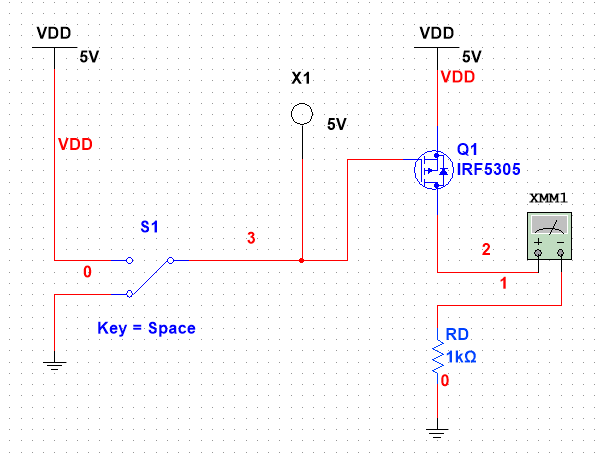
\includegraphics[width=10cm]{1}
\caption*{\textbf{Rys. 17}: Schemat obwodu elektrycznego z tranzystorem PMOS oraz przełącznikiem. }
\end{figure}
\noindent Dołączony multimetr $XMM1$ pozwala sprawdzić prąd w obwodzie drenu. Na wyjściu będzie sygnał wysoki 1 jeżeli w obwodzie drenu będzie płynął prąd rzędu $mA$ za sygnał 0 jeśli prąd rzedu ${\mu}A$. Na \textbf{Rys. 18} widać wyniki
pomiaru dla sygnału wysokiego na wejściu. Prąd rzedu ${\mu}A$ pokazuje, że na wyjściu mamy sygnał 0. Wyniki reszty pomiarów pokazane są w tabeli na \textbf{Rys. 19}.
\begin{figure}[H]
\centering
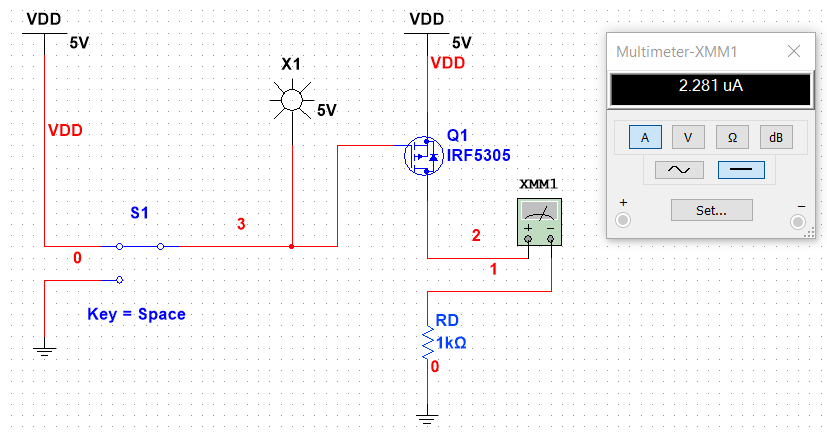
\includegraphics[width=10cm]{3}
\caption*{\textbf{Rys. 18}: Wyniki pomiaru prądu na drenie dla sygnału wejściowego 1 - sygnał 0 na wyjściu. }
\end{figure}
\begin{figure}[H]
\centering
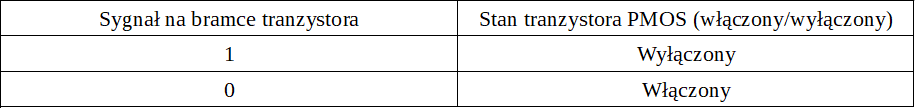
\includegraphics[width=10cm]{7}
\caption*{\textbf{Rys. 19}: Tabela pokazująca zależność sygnału wyjściowego od sygnału wejściowego w obwodzie. }
\end{figure}
\noindent W obwodzie wymieniłem tranzystor unipolarny PMOS na NMOS oraz wykonałem takie same działania jak wcześniej. Układ widoczny jest na \textbf{Rys. 20} .Na \textbf{Rys. 21} widać wyniki pomiaru dla sygnału wysokiego na wejściu. Prąd rzedu $mA$ pokazuje, że na wyjściu mamy sygnał 1. Wyniki reszty pomiarów pokazane są w tabeli na \textbf{Rys. 22}.
\begin{figure}[H]
\centering
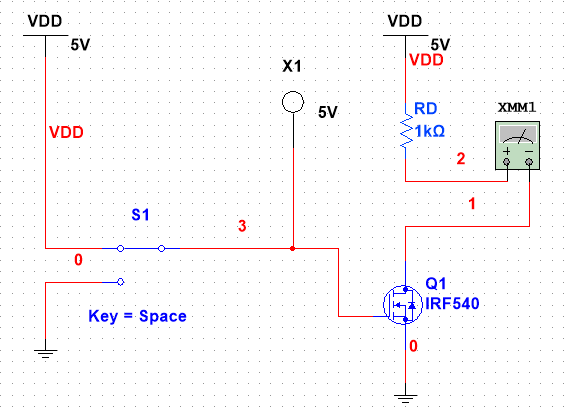
\includegraphics[width=10cm]{4}
\caption*{\textbf{Rys. 20}: Schemat obwodu elektrycznego z tranzystorem NMOS oraz przełącznikiem.}
\end{figure}
\begin{figure}[H]
\centering
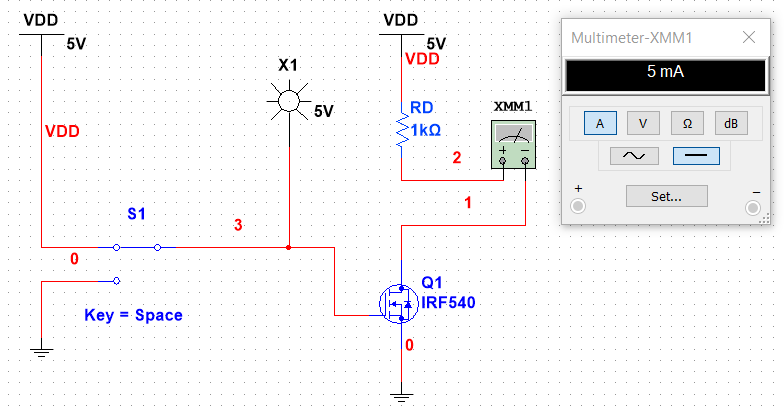
\includegraphics[width=10cm]{6}
\caption*{\textbf{Rys. 21}: Wyniki pomiaru prądu na drenie dla sygnału wejściowego 1 - sygnał 1 na wyjściu. }
\end{figure}
\begin{figure}[H]
\centering
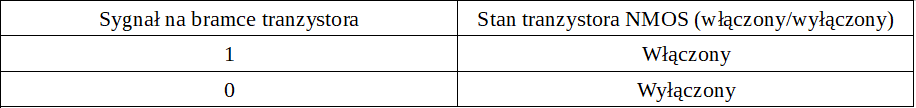
\includegraphics[width=10cm]{8}
\caption*{\textbf{Rys. 22}: Tabela pokazująca zależność sygnału wyjściowego od sygnału wejściowego w obwodzie. }
\end{figure}
\subsection{Wnioski}
Wykonane ćwiczenie pokazuje, że układy tranzystorów można skutecznie używać do prostych układów logicznych dzięki czemu możemy manipulować sygnałem na wyjściu przy użyciu sygnału wejściowego.
\section{Inwerter logiczny}
\subsection{Cel ćwiczenia}
Celem ćwiczenia było zapoznanie się z prostym układem logicznym inwertera logicznego zbudowanym z tranzystora NMOS i PMOS oraz sprawdzenie stanu tranzystorów w zależności od napięcia podanego na bramkę.
\subsection{Przebieg ćwiczenia}
Na pulpicie symulacyjnym zbudowałem obwód elektryczny inwertera logicznego zawierający źródła napięcia $V_{DD}=5V$, przełącznika podającego na bramkę tranzystora sygnał wysoki 1 o amplitudzie $5V$ lub sygnał niski $0V$. Sprawdziłem jego zachowanie
po podaniu wysokiego i niskiego sygnału na bramkę. Układ widoczny jest na \textbf{Rys. 23}.
\begin{figure}[H]
\centering
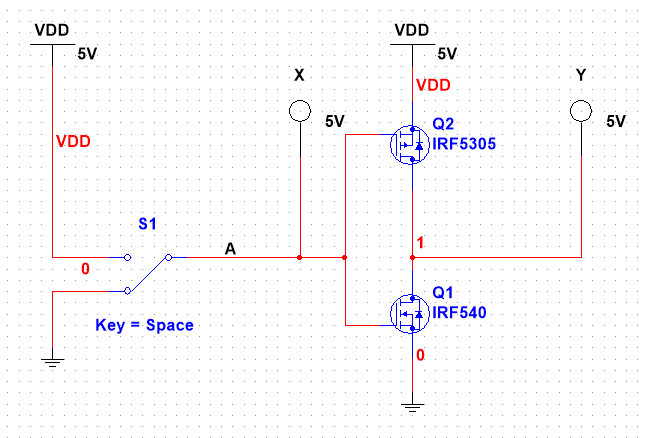
\includegraphics[width=10cm]{9}
\caption*{\textbf{Rys. 23}: Schemat obwodu elektrycznego inwertera logicznego z przełącznikiem. }
\end{figure}
\noindent Na \textbf{Rys. 24} widać wyniki pomiaru dla sygnału niskiego na wejściu. Lampka sygnalizacyjna na wyjściu wskazuje, że mamy sygnał wysoki na wyjściu. Wyniki reszty pomiarów pokazane są w tabeli na \textbf{Rys. 25}.
\begin{figure}[H]
\centering
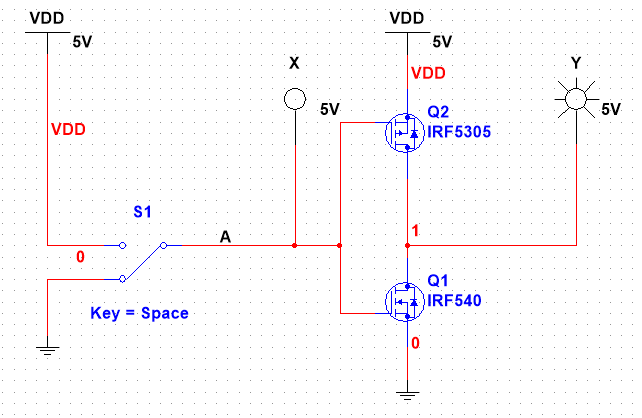
\includegraphics[width=10cm]{10}
\caption*{\textbf{Rys. 24}: Wyniki pomiaru prądu na drenie dla sygnału niskiego 0 - sygnał 1 na wyjściu. }
\end{figure}
\begin{figure}[H]
\centering
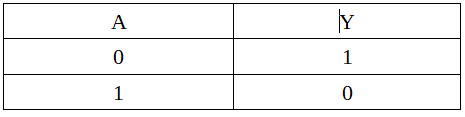
\includegraphics[width=10cm]{12}
\caption*{\textbf{Rys. 25}: Tabela pokazująca zależność sygnału wyjściowego od sygnału wejściowego w obwodzie inwertera logicznego.}
\end{figure}
\subsection{Wnioski}
Wykonane ćwiczenie pokazuje, że układy tranzystorów można skutecznie używać jako inwertera logicznego. Tabelka prawdy widoczna na \textbf{Rys. 25} pokazuje, że zastosowany układ jest poprawny.
\section{Bramka NAND}
\subsection{Cel ćwiczenia}
Celem ćwiczenia było zapoznanie się z prostym układem logicznym bramki NAND zbudowanym z tranzystorów NMOS i PMOS oraz sprawdzenie stanu tranzystorów w zależności od napięcia podanego na bramkę.
\subsection{Przebieg ćwiczenia}
Na pulpicie symulacyjnym zbudowałem obwód elektryczny bramki NAND zawierający źródła napięcia $V_{DD}=5V$, przełączników podających na bramkę tranzystora kombinację sygnałów niskim 0 i wysokich 1. Sprawdziłem jego zachowanie
po podaniu wszystkich kombinacji sygnałów na wejściu. Układ widoczny jest na \textbf{Rys. 26}.
\begin{figure}[H]
\centering
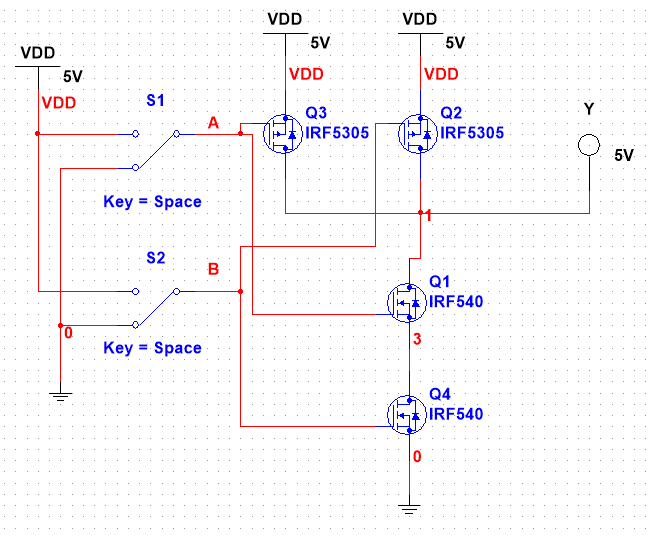
\includegraphics[width=10cm]{13}
\caption*{\textbf{Rys. 26}: Schemat obwodu elektrycznego bramki NAND z przełącznikami. }
\end{figure}
\noindent Na \textbf{Rys. 27} widać wyniki pomiaru dla sygnału niskiego na wejściu A oraz sygnału wysokiego na wejściu B. Lampka sygnalizacyjna na wyjściu wskazuje, że mamy sygnał wysoki na wyjściu. Wyniki reszty pomiarów pokazane są w tabeli na \textbf{Rys. 28}.
\begin{figure}[H]
\centering
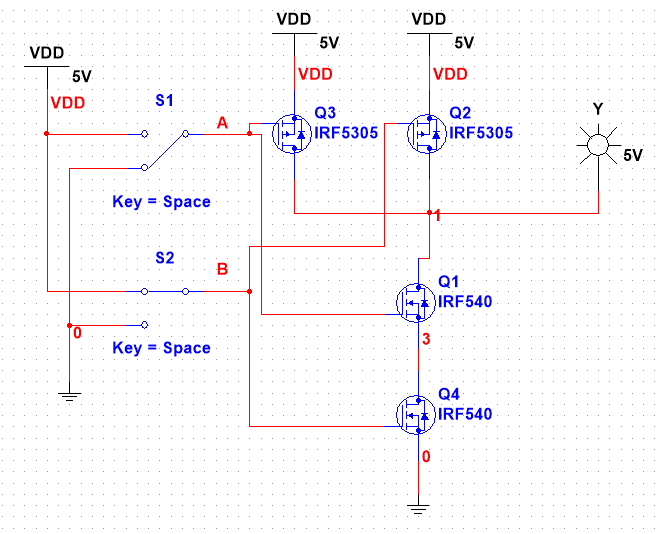
\includegraphics[width=10cm]{15}
\caption*{\textbf{Rys. 27}: Wyniki pomiaru prądu na drenie dla sygnału niskiego na wejściu A oraz sygnału wysokiego na wejściu B - sygnał 1 na wyjściu. }
\end{figure}
\begin{figure}[H]
\centering
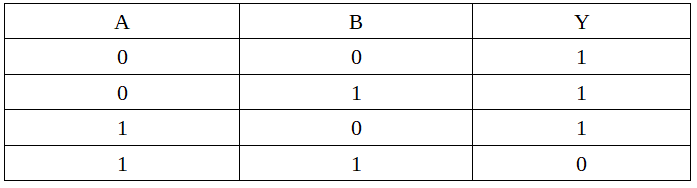
\includegraphics[width=10cm]{18}
\caption*{\textbf{Rys. 28}: Tabela pokazująca zależność sygnału wyjściowego od sygnałów wejściowych w obwodzie bramki NAND.}
\end{figure}
\subsection{Wnioski}
Wykonane ćwiczenie pokazuje, że układy tranzystorów można skutecznie używać jako bramki NAND. Tabelka prawdy widoczna na \textbf{Rys. 28} pokazuje, że zastosowany układ jest poprawny.
\section{Bramka AND}
\subsection{Cel ćwiczenia}
Celem ćwiczenia było zapoznanie się z prostym układem logicznym bramki AND zbudowanym z tranzystorów NMOS i PMOS i inwertera logicznego oraz sprawdzenie stanu tranzystorów w zależności od napięcia podanego na bramkę.
\subsection{Przebieg ćwiczenia}
Na pulpicie symulacyjnym zbudowałem obwód elektryczny bramki AND zawierający źródła napięcia $V_{DD}=5V$, przełączników podających na bramkę tranzystora kombinację sygnałów niskim 0 i wysokich 1. Sprawdziłem jego zachowanie
po podaniu wszystkich kombinacji sygnałów na wejściu. Układ widoczny jest na \textbf{Rys. 29}.
\begin{figure}[H]
\centering
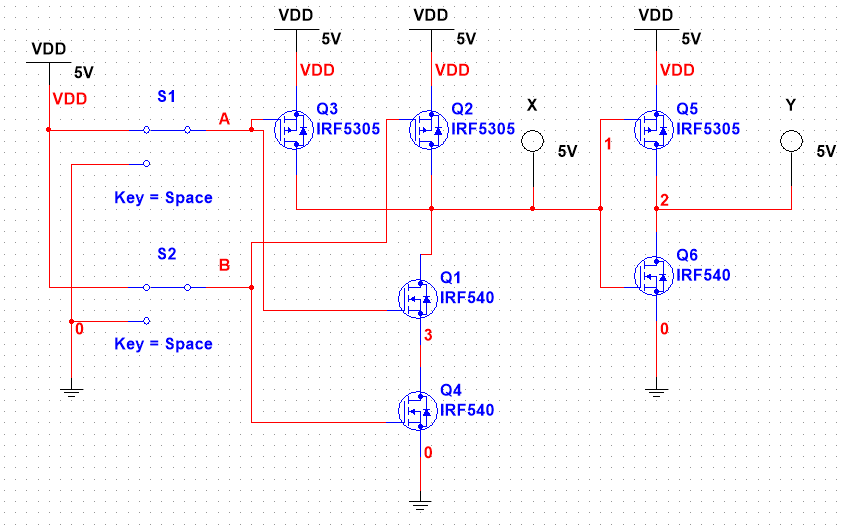
\includegraphics[width=10cm]{19}
\caption*{\textbf{Rys. 29}: Schemat obwodu elektrycznego bramki AND z przełącznikami. }
\end{figure}
\noindent Na \textbf{Rys. 30} widać wyniki pomiaru dla sygnału niskiego na wejściu A oraz sygnału wysokiego na wejściu B. Lampka sygnalizacyjna na wyjściu wskazuje, że mamy sygnał niski na wyjściu. Wyniki reszty pomiarów pokazane są w tabeli na \textbf{Rys. 31}.
\begin{figure}[H]
\centering
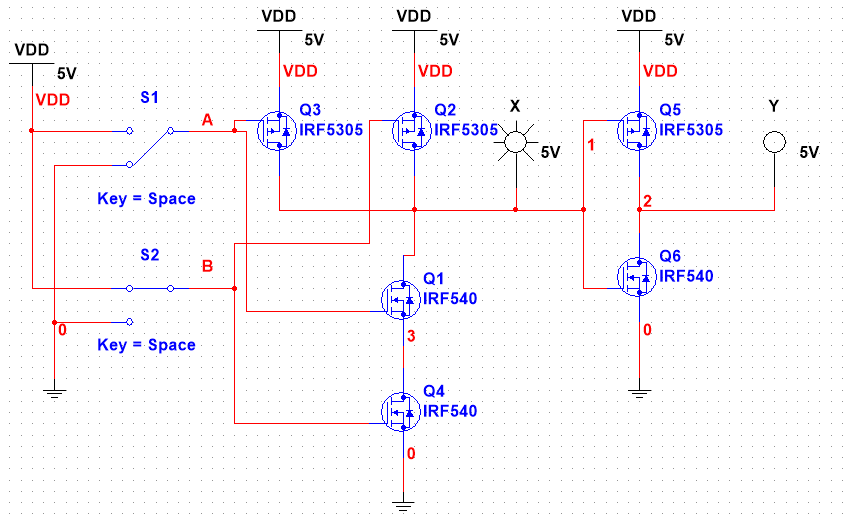
\includegraphics[width=10cm]{21}
\caption*{\textbf{Rys. 30}: Wyniki pomiaru prądu na drenie dla sygnału niskiego na wejściu A oraz sygnału wysokiego na wejściu B - sygnał 0 na wyjściu. }
\end{figure}
\begin{figure}[H]
\centering
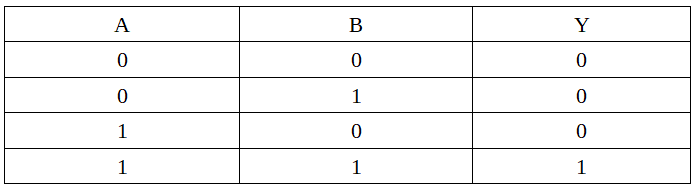
\includegraphics[width=10cm]{24}
\caption*{\textbf{Rys. 31}: Tabela pokazująca zależność sygnału wyjściowego od sygnałów wejściowych w obwodzie bramki AND.}
\end{figure}
\subsection{Wnioski}
Wykonane ćwiczenie pokazuje, że układy tranzystorów można skutecznie używać jako bramki AND. Bramkę AND można otrzymać łącząc obwód bramki NAND z inwerterem logicznym. Tabelka prawdy widoczna na \textbf{Rys. 31} pokazuje, że zastosowany układ jest poprawny.
\section{Bramka NOR}
\subsection{Cel ćwiczenia}
Celem ćwiczenia było zapoznanie się z prostym układem logicznym bramki NOR zbudowanym z tranzystorów NMOS i PMOS oraz sprawdzenie stanu tranzystorów w zależności od napięcia podanego na bramkę.
\subsection{Przebieg ćwiczenia}
Na pulpicie symulacyjnym zbudowałem obwód elektryczny bramki NOR zawierający źródła napięcia $V_{DD}=5V$, przełączników podających na bramkę tranzystora kombinację sygnałów niskim 0 i wysokich 1. Sprawdziłem jego zachowanie
po podaniu wszystkich kombinacji sygnałów na wejściu. Układ widoczny jest na \textbf{Rys. 32}.
\begin{figure}[H]
\centering
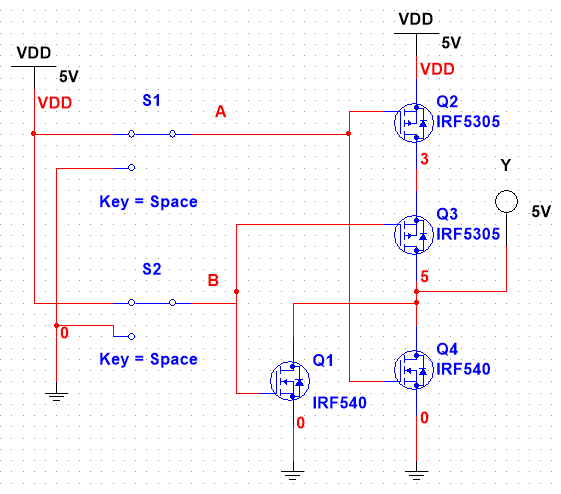
\includegraphics[width=10cm]{25}
\caption*{\textbf{Rys. 32}: Schemat obwodu elektrycznego bramki NOR z przełącznikami. }
\end{figure}
\noindent Na \textbf{Rys. 33} widać wyniki pomiaru dla sygnału niskiego na wejściu A oraz sygnału wysokiego na wejściu B. Lampka sygnalizacyjna na wyjściu wskazuje, że mamy sygnał niski na wyjściu. Wyniki reszty pomiarów pokazane są w tabeli na \textbf{Rys. 34}.
\begin{figure}[H]
\centering
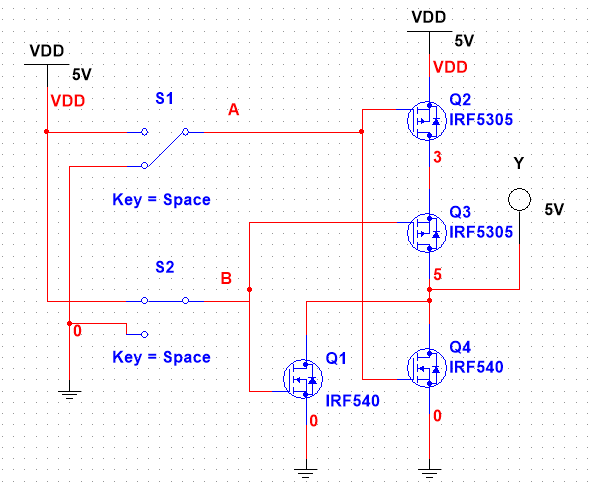
\includegraphics[width=10cm]{27}
\caption*{\textbf{Rys. 33}: Wyniki pomiaru prądu na drenie dla sygnału niskiego na wejściu A oraz sygnału wysokiego na wejściu B - sygnał 0 na wyjściu. }
\end{figure}
\begin{figure}[H]
\centering
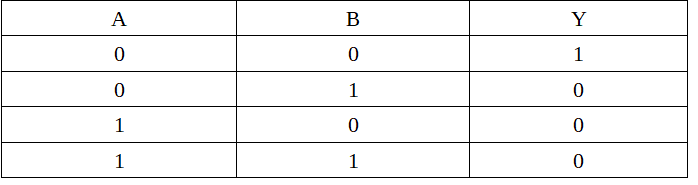
\includegraphics[width=10cm]{30}
\caption*{\textbf{Rys. 34}: Tabela pokazująca zależność sygnału wyjściowego od sygnałów wejściowych w obwodzie bramki NOR.}
\end{figure}
\subsection{Wnioski}
Wykonane ćwiczenie pokazuje, że układy tranzystorów można skutecznie używać jako bramki NOR. Tabelka prawdy widoczna na \textbf{Rys. 34} pokazuje, że zastosowany układ jest poprawny.
\section{Bramka OR}
\subsection{Cel ćwiczenia}
Celem ćwiczenia było zapoznanie się z prostym układem logicznym bramki OR zbudowanym z tranzystorów NMOS i PMOS i inwertera logicznego oraz sprawdzenie stanu tranzystorów w zależności od napięcia podanego na bramkę.
\subsection{Przebieg ćwiczenia}
Na pulpicie symulacyjnym zbudowałem obwód elektryczny bramki OR zawierający źródła napięcia $V_{DD}=5V$, przełączników podających na bramkę tranzystora kombinację sygnałów niskim 0 i wysokich 1. Sprawdziłem jego zachowanie
po podaniu wszystkich kombinacji sygnałów na wejściu. Układ widoczny jest na \textbf{Rys. 35}.
\begin{figure}[H]
\centering
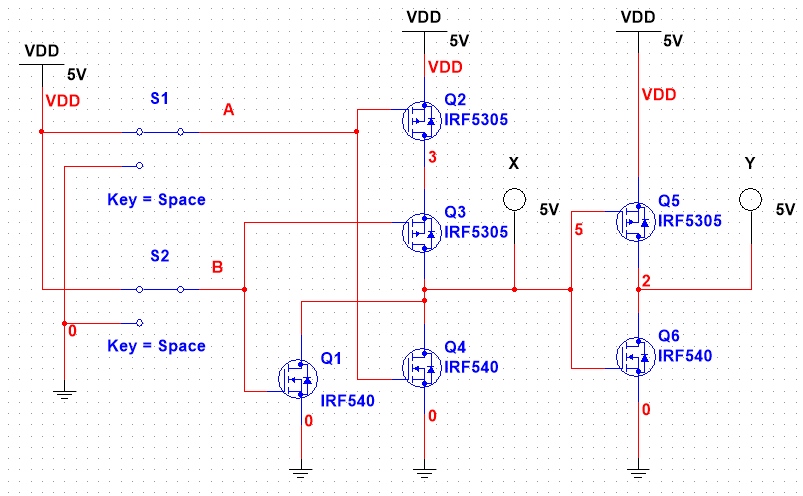
\includegraphics[width=9cm]{31}
\caption*{\textbf{Rys. 35}: Schemat obwodu elektrycznego bramki OR z przełącznikami. }
\end{figure}
\noindent Na \textbf{Rys. 36} widać wyniki pomiaru dla sygnału niskiego na wejściu A oraz sygnału wysokiego na wejściu B. Lampka sygnalizacyjna na wyjściu wskazuje, że mamy sygnał wysoki na wyjściu. Wyniki reszty pomiarów pokazane są w tabeli na \textbf{Rys. 37}.
\begin{figure}[H]
\centering
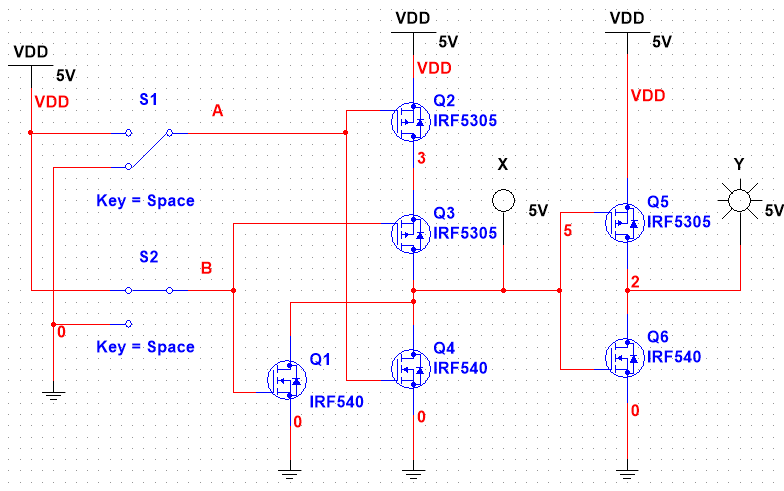
\includegraphics[width=9cm]{33}
\caption*{\textbf{Rys. 36}: Wyniki pomiaru prądu na drenie dla sygnału niskiego na wejściu A oraz sygnału wysokiego na wejściu B - sygnał 1 na wyjściu. }
\end{figure}
\begin{figure}[H]
\centering
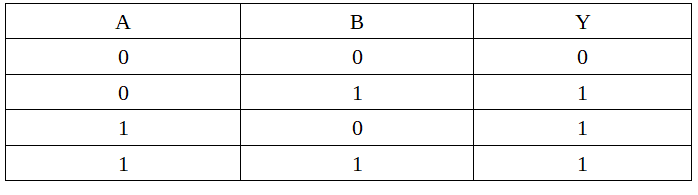
\includegraphics[width=10cm]{36}
\caption*{\textbf{Rys. 37}: Tabela pokazująca zależność sygnału wyjściowego od sygnałów wejściowych w obwodzie bramki OR.}
\end{figure}
\subsection{Wnioski}
Wykonane ćwiczenie pokazuje, że układy tranzystorów można skutecznie używać jako bramki OR. Bramkę OR można otrzymać łącząc obwód bramki NOR z inwerterem logicznym. Tabelka prawdy widoczna na \textbf{Rys. 37} pokazuje, że zastosowany układ jest poprawny.
\end{document}